
\label{sec:systemArchitecture}

Dieses Kapitel soll ein Gefühl für die Komponenten von \emph{Flewnit} und 
ihre Zusammenhänge vermitteln. Die Komponenten "`in Aktion"' werden im Detail im Verlauf des Kapitels 
\ref{sec:simulation} beschrieben.

Das System wurde in C++ als (wahlweise statisch oder dynamisch zu linkende) Bibliothek implementiert.
Der Code der GPU-Programme ist in GLSL bzw. OpenCL C verfasst.

\subsection{Dependencies}
	\label{sec:dependencies}
	
	Zunächst sollen die verwendeten Third-Party-Bibliotheken kurz vorgestellt werden:

	\begin{description}
		\item[OpenGL3/4]
		Die schon mehrfach erwähnten modernen Versionen der \linebreak \emph{Open Graphics Library},
		der offenen API der Khronos Group zur \linebreak hardwarebeschleunigten Graphik-Programmierung 
		auf Basis der Dreiecks-Rasterisierung.
		\todo[color=green]{evtl treffenderen Ausdruck finden: Scanline-basiert oder was auch immer}
		Um die Programmierung ohne Legacy-Routinen nicht erst zur Laufzeit über einen OpenCL-Error
		durch Verwendung eines Core-Profiles zu erzwingen, gibt es einen OpenGL- Header
		namens "`gl3.h"'\footnote{beziehbar unter http://www.opengl.org/registry/},
		der in Kombination mit der entsprechenden Präprozessor-Definition
		\lstinline[language=C]|#define GL3_PROTOTYPES 1| schon zur Compile-Zeit nur die non-deprecated
		Routinen zur Verfügung stellt.
		
     	\item[OpenCL 1.0]
	    Die \emph{Open Computing Language}, erste Version der noch jungen API für massiv parallele Programmierung
	    \footnote{die GPGPU-Computing einschließt}, wie OpenGL von der Khronos Group verwaltet; 
	    sie stellt den ersten offenen Standard für GPGPU dar, d.h., die Verwendung der API ist nicht mehr an eine
	    bestimmte Hardware (wie bei Nvidia CUDA) oder ein bestimmtes Betriebssystem (wie Microsofts DirectCompute)
	    gebunden.
	    
	    Zur Zeit der Implementierung waren noch keine Non-Developer-Treiber für OpenCL 1.1 verfügbar, 
	    außerdem gab es kein Feature dieser Version, welches ich dringend benötigt hätte.
	    Deshalb habe ich die Version 1.0 verwendet.
	    
	    Es gibt einen C++ -Wrapper der C-API, welcher stark auf C++-Templates basiert und in einer einzigen Headerdatei 
	    implementiert ist. Dieser ist direkt von der Khronos-Homepage\footnote{http://www.khronos.org/registry/cl/} 	
	    beziehbar. Diesen Wrapper habe ich verwendet, da er die Nutzung der API wesentlich eleganter macht.
	    
    	
   		\item[GLFW 2.7]
		Wie auf Seite \pageref{focus:dependencies} angedeutet, waren mir folgende Dinge wichtig, damit die Einsetzbarkeit
		des Frameworks in professionelleren Kontexten nicht schon im Vorfeld verbaut ist:
		\begin{itemize}
			\item Option auf Fullscreen
			\item Option auf Multisampling
			\item Die Möglichkeit der Erstellung eines OpenGL-Kontextes einer frei wählbaren Version 
			mit Option zwischen Core- und Compatibility-Profile
			\item Option auf "`\emph{Mouse Grab}"', so dass man wie in einem Computerspiel mit ausgeblendetem Mauszeiger
			nur durch Bewegung der Maus ohne Bildschirm-/Fenster-Grenzen die virtuelle Kamera rotieren kann;
			\item "`Input events"', d.h. Aktualisierungen von Benutzereingaben sollen häufig und mit minimaler 
			Latenz geschehen, außerdem so unabhängig wie möglich von der Framerate sein;
			Nach möglichkeit sollten Input-Updates zumindest "aktiv abfragbar" sein 
			(im Gegensatz zum passiven Warten darauf, dass von der Input-Library eine Callback-Funktion 
			aufgerufen wird)
			\item Es soll volle Kontrolle über die "Render-Loop" geben, so dass man nicht 
			den Kontrollfluss an eine Funktion übergibt, die womöglich nie zurückkehrt und weiteren Kontrollfluss
			durch das Benutzerprogramm	nur über Callback-Funktionen ermöglicht
			(wie \lstinline[language=C]|glutEnterMainLoop()| beim in die Jahre gekommenen \emph{GLUT}).
			Ein derartiges Konstrukt ist einer
			Engine nicht würdig und verhindert womöglich sauberes Herunterfahren und Neu-Initialisierung,
			wie es z.B. beim Wechseln einer Szene oder eines fundamentalen globalen Settings nötig sein könnte.	
		\end{itemize}
		\emph{GLFW}\footnote{http://www.glfw.org/} in der Version 2.7, die zum Zeitpunkt der Implementation aktuellste 
		stabile	Version, erfüllt diese Forderungen, und findet damit in \emph{Flewnit} Einsatz sowohl im Fenster- als auch 	
		im Input-Manager. Die Timing-Funktionalität wird ebenfalls von GLFW übernommen.
		
    	
    	\item[OpenGL Mathematics (GLM)]
    	Seit sämtlicher Mathematik-bezogener OpenGL-State inklusive zugehöriger built-in-Variablen und -Funktionen
    	wie \lstinline[language=GLSL]|gl_ModelViewProjectionMatrix| oder
    	\lstinline[language=GLSL]|ftransform()|
    	in GLSL abgeschafft wurden, führt um eine Bibliothek für Vektor- und Matrix-Algebra kein Weg mehr herum.
    	Ich habe mich für \emph{GLM}\footnote{http://glm.g-truc.net/} entschieden, da sie klein und dennoch mächtig ist,
    	und einige Convenience-Functions hat; QT hat ebenfalls eine Mathe-Bibliothek, verwendet jedoch
    	\lstinline[language=C]|double|, also 64bit-Fließkomma-Werte als Basis-Datentyp, was das direkte Übergeben
    	als Array von \lstinline[language=C]|float|-Uniforms an die OpenGL-Shader verhindert. Zwar unterstützen OpenGL
    	und moderne Graphikkarten \lstinline[language=C]|double| nativ, jedoch mit drastisch geringerer Geschwindigkeit,
    	da weniger Recheneinheiten für diesen Datentypen zur Vervügung stehen.\\
    	Es sei bemerkt, dass ich persönlich die direkte Verwendung einer C++ - Mathe-Bibiothek mit überladenen Operatoren
    	und eigener Akkumulation von Matrizen wesentlich angenehmer und eleganter finde als das zähe Hantieren
    	mit der C-API zum modifizieren des OpenGL-State mit seinen Matrix-Modes.
    	
    	\item[Grantlee]
	 		\lstset{language=GLSL} 
       		Die bereits erwähnte Template-Engine; die Syntax entspricht der der Template-Sprache des 
       		\emph{Django} web Frameworks\footnote{https://www.djangoproject.com/}.\\

       		Es lassen sich durch die Applikation Werte an die Template-Engine übergeben, anhand derer
       		dann die Code-Generierung Kontrolliert wird, bzw welche durch durch Einschluss in doppelte
       		geschwungene Klammern direkt eingefügt werden können. \\
       		Beipiel:
			\begin{lstlisting}      		
vec4 fragmentColor =  	
	  
		texture(decalTexture,input.texCoords.xy);
	 color;
	  
			\end{lstlisting} 
			\begin{lstlisting}
#define NUM_BITS_PER_KEY_TO_SORT ( {{numBitsPerKey}} )
			\end{lstlisting} 
     		
       		Die Engine stellt einen Vererbungs-Mechanismus bereit:\\
       		Auf diese Weise kann z.B. die Datei "`particleSimulationTemplate.cl"' verschiedene "`Code-Blocks"'
       		definieren wie z.B.
       		
       		\begin{lstlisting}

	
	the core of the physics simulation: 
	accumulate all relevant values 
	(density, pressure force, viscosity force etc ...)
	               

       		\end{lstlisting}
       		
       		, die von anderen Datein geerbt und entsprechend angepasst implementiert werden.\\
       		"`updateDensity.cl"' erbt von dieser Datei durch die Directive
       		\lstinline[language=GLSL]|| 
       		und implementiert die Dichte-Berechnungen, 
       		ohne dass der umschließende (nicht unerheblich lange und komplexe) Kontrollfluss-Code wiederholt werden muss:
       		\begin{lstlisting}

	if( BELONGS_TO_FLUID(
			GET_CURRENT_NEIGHBOUR_PARTICLE_OBJECT_ID  ) )
	{
		ownDensity +=                   
			cObjectGenericFeatures [ GET_CURRENT_NEIGHBOUR_PARTICLE_OBJECT_ID  ].massPerParticle
			* poly6( ownPosition -  GET_CURRENT_NEIGHBOUR_POS , cSimParams );
	}

       		\end{lstlisting}

       		
       		
    	\item[Assimp]
    	Die \emph{Open Asset Import Library}\footnote{http://assimp.sourceforge.net/} ermöglicht das Auslesen
    	von Szenen direkt aus .blend-Dateien, dem nativen Datenformat des exzellenten Free Software -- 3D-
    	Modellierungsprogramms \emph{Blender}\footnote{http://www.blender.org/}.
    	Somit entfällt der Umständliche Export in ein Zwischenformat.

    	
   		\item[TinyXML]
   		Um zu gewährleisten, dass das System schon in der frühen Entwicklungsphase weitgehend ohne 
   		Recompile-benötigenden "`Hard-Codes"' konfigurierbar ist, wurde TinyXML verwended, um eine XML-
   		config-Datei zu parsen.    	
    
	
	\end{description}	

	Außerdem haben manche Komponenten der \emph{Boost}-Libraries\footnote{http://www.boost.org/} verwendet.
	
	


\subsection{Klassendiagramm}
Abbildung \ref{fig:ClassDiagOverview1} und \ref{fig:ClassDiagOverview2} zeigen ein vereinfachtes Klassendiagramm
von \emph{Flewnit}. Die roten Klassen stellen wichtige Meta-Informationen dar, um Kontrollfluss und Objekt-Erstellung
zu delegieren. In den folgenden Unterabschnitten werden die einzelnen Komponenten detaillierter vorsgestellt.

\begin{figure}[!h]
	 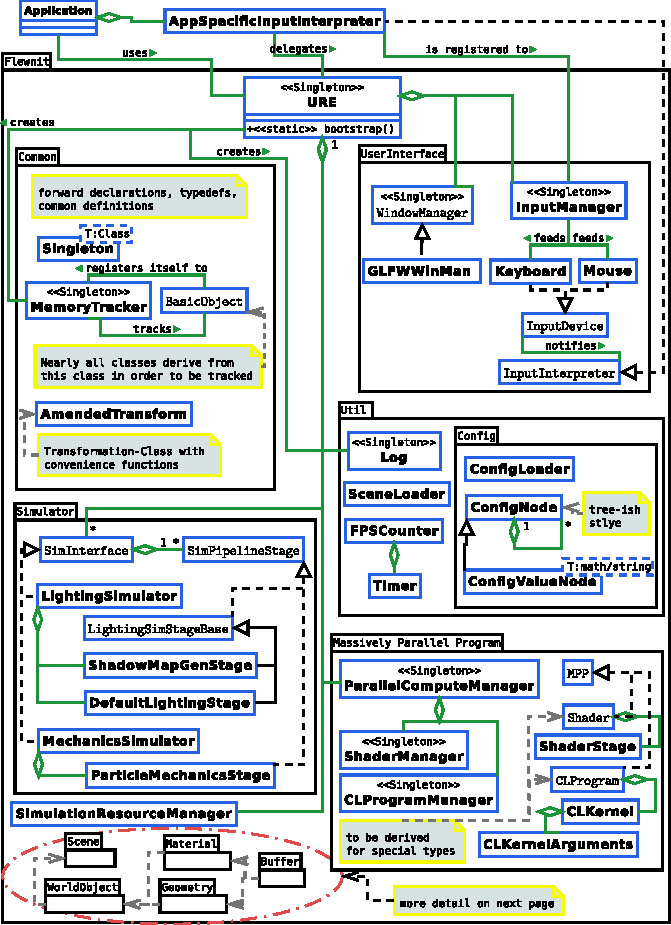
\includegraphics[width=1.15\textwidth]{Overview_Flewnit_Architecture_After_Implementation1.pdf}
	\caption{Klassendiagramm des Gesamtsystems, Teil 1}
	\label{fig:ClassDiagOverview1}
\end{figure}


\begin{figure}[!h]
	 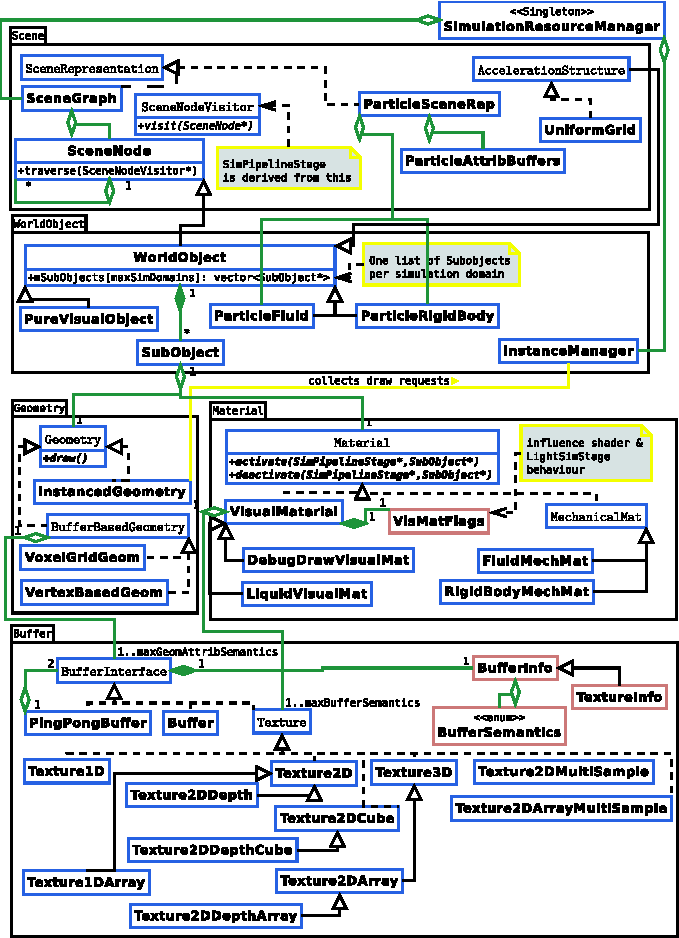
\includegraphics[width=1.15\textwidth]{Overview_Flewnit_Architecture_After_Implementation2.pdf}
	\caption{Klassendiagramm des Gesamtsystems, Teil 2}
	\label{fig:ClassDiagOverview2}
\end{figure}



 
\subsection{BasicObject und Memory Tracking}
	\lstset{language=C++} %we want c++ code listings
	
	Die Bibliothek soll zur Laufzeit kontrolliert herunterfahr- und re-initialisier-bar sein, 
	um eine vielseitige und flexible Anwendung zu gewährleisten. Da bei C++ das Speicher-Management dem
	Programmierer überlassen ist, und man daher vor allem bei massiver Nutzung von Pointern schnell den Überblick
	verliert, 
	\begin{itemize}
		\item welches Objekt welche anderen erschaffen hat
		\item welche Objekte eine Klasse "`besitzt"' und somit für ihre Speicher-Freigabe zuständig ist bzw
		\item auf welche Objekte eine Klasse nur ein Handle für Verwaltung oder	Backtracking hat, ohne für Erschaffung
		 oder Löschung zuständig zu sein
	\end{itemize}
	wurde in Anbetracht der oberen Forderung ein sehr simples Meta-Object-System system realisiert, welches Klassen-Namen
	und Speicherverbrauch eines Objektes feststellt sowie jedem Objekt eine \emph{unique ID} zuweist.
	Zweck dieses Meta Object System-Systems war es, Speicherlecks durch Nicht-Löschen von Objekten während der Entwicklung 
	zu finden;
	
	Dafür erbt beinahe jede Klasse in \emph{Flewnit} von \lstinline|BasicObject|.
	Diese Klasse registriert sich automatisch bei der \lstinline|MemoryTracker|-Singleton-Instanz, bekommt dort eine
	ID zugewiesen. Diese ID hat noch keine Anwendung, könnte sich aber in einem Netzwerk-Kontext als nützlich erweisen.

	Wie bei Qt das \lstinline[language=C++]|Q_OBJECT|-Makro muss in jede von 
	\lstinline[language=C++]|BasicObject| erbende Klasse das Makro 
	\lstinline[language=C++]|FLEWNIT_BASIC_OBJECT_DECLARATIONS| eingetragen werden; Dieses Makro definiert die 
	Implementatoin einer virtuellen Funktion, welche die Meta-Information setzen:
    \begin{lstlisting}
#define FLEWNIT_BASIC_OBJECT_DECLARATIONS \
	public:\
		virtual void initBasicObject() \
		{ \
			mMemoryFootPrint = (int) sizeof(*this); \
			mClassName = String(typeid(*this).name()); \
		} \
	private:	
	\end{lstlisting}
	Diese umständliche Implementierung hat die Urasache, dass Typ-Informationen der Blatt-Klasse einer
	Klassenhierarchie erst dann zur verfügung stehen, wenn alle Konstruktoren der Basis-Klassen zurückgekehrt sind,
	weshalb der obere Code also nicht im Konstruktor der Basisklasse stehen darf, da der \lstinline|this|-Pointer
	noch nicht die Informationen der Blatt-Klasse enthält.
	Ferner, um dem Programmierer nicht zuzumuten, \lstinline|initBasicObject()| in jedem Konstruktor aufzurufen
	(das führt bei tiefen Klassenhierarchien zu unnötigen ausführungen dieser Funktion, da nur die Info der Blatt-Klasse
	benötigt wird, außerdem entstünde so eine weitere Vergesslichkeits-Fehlerquelle, die durch das Meta Object System ja 
	gerade \emph{vermieden} werden soll), stellt der Memory Tracker eine Routine \lstinline|updateMemoryTrackingInfo()|
	bereit, die aufgerufen werden sollte, wenn man auf valide Meta-Information zugreifen will.
	Aufpassen muss man bei tiefen Klassenhierarchien, da hier der Compiler keinen Fehler erzeugt, wenn eine Blatt-Klasse
	das Makro nicht eingetragen hat, da eine Implementierung der Funktion ja bereits durch eine Oberklasse existiert.
	
	Über bedingte Kompilierung lässt sich diese Meta-Funktionalität deaktivieren.
	Ein "`richtiges"' Meta Object System wie das von Qt wollte ich nicht verwenden, da es für meine Zwecke zu komplex und
	mächtig ist, und ich nicht mit Kanonen auf Spatzen schießen wollte. Ohnehin gibt es Tools wie Valgrind, mit denen
	man Speicherlecks finden kann. 

	Letztendlich ist meine Lösung nicht wirklich elegant (auch wenn ich ohne Meta-Object-Compiler (MOC) keine bessere 	
	Lösung gefunden habe) und daher eher als eine Spielerei anzusehen
	mit dem Zwecke, die C++-Interna zu verinnerlichen und zu jeder Zeit daran erinnert zu werden, 
	Destruktoren zu implementieren und sich über 
	"`Besitz- und Verwaltungs-Verhältnisse"' der Klassen Gedanken zu machen.
	
	Der \lstinline|MemoryTracker| verfolgt auch sämtliche Allokationen der \lstinline|BufferInterface|-Klasse,
	also der Basisklasse sämtlicher Buffer-Typen;
	
\subsection{AmendedTransform}
	\label{sec:AmendedTransform}
 	Im Zuge der Überlegungen zum Szenegraphen, der Kamera und des visuellen Renderings vieler Objekte per
 	Hardware-Instancing entschied ich mich, die klassische 4x4-Transformationsmatrix zu wrappen und mit
 	convenience functions anzureichern, siehe Listing \ref{listing:AmendedTransformDef}.\\
 	Der Zweck dieser Klasse ist es, Transformationsmatrizen anhand "`anschaulicher"' Parameter 
 	(Position, Richtung, Up-Vektor, Skalierung) zu definieren,
 	und diese Parameter auch nach Akkumulationen, Modifikationen und/oder Animationen zur Verfügung zu haben.\\
 	Der Fokus liegt hier klar auf der Bequemlichkeit für den Entwickler, nicht auf der Performanz.
 	Sobald sehr große, dynamisch animierte und tiefe Scenegraphen zum Einsatz kommen, könnte diese Klasse
 	zum Flaschenhals werden. Dann ist vielleicht ein Refactoring vonnöten; Vorerst scheint mir die Implementation jedoch
 	angemessen.\\
 	
 	So lässt sich z.B. bequem ein \lstinline|Camera|-Objekt, welches selber von \lstinline|WorldObject| erbt,
 	welches wiederum von \lstinline|SceneNode| abgeleitet ist, an eine andere SceneNode anhängen, und aus der automatisch
 	berechneten globalen Transformation erhält man durch \lstinline|AmendedTransform::getLookAtMatrix()|
 	direkt die lookAt-Matrix, so  dass die Camera-Klasse selber sich nur noch um seine Projektionsmatrix kümmern muss.
 	Auch typische Animationen werden von der Klasse übernommen. Ob dies guter Stil ist, oder doch lieber in die
 	SceneNode-Klasse ausgelagert werden sollte, ist eine Frage, die ich noch nicht abschließend beantworten kann.
 	Es wurde hier dem Paradigma der Datenlokalität gefolgt, evtl. auf Kosten der Separation of Concerns.
 	Eine weitere Erörtertung lasse ich aus, da das Refactoring in diesem Falle nicht zu aufwändig wäre;

	Es sei bemerkt, dass durch die Menge an Matrizen, die an den Vertex Shader beim Instanced Rendering übergeben
	werden müssen, wenn man für alle Fälle gewappnet sein will
	\footnote{z.B. für Layered Rendering in verschiedene Texturen, z.B in ein Textur-Array zur Generierung mehrerer 
	Spotlight-Shadowmaps mit einem Draw-Call; Hierbei braucht es explizit nur die Model-Matrix, da es pro Layer 
	verschiedene View-Matrices (pro Spotlight eine) gibt, von daher nicht im Vorfeld eine ModelView Matrix akkumuliert 
	werden kann}, nicht unerheblich ist, da für jede Instanz ein anderes Matrix-Set übergeben werden muss;
	Die Menge an Daten, die per Uniform-Variable übergeben werden kann, ist begrenzt, daher hängt die maximale Anzahl
	an Instanzen, die pro Draw-Call gezeichnet werdne können, direkt davon ab, wie viele Daten pro Instanz übergeben 
	werden müssen;\\
	Dieser Umstand hat mich dazu verleitet, die Normal Matrix, die transponierte Inverse der ModelView-Matrix,
	"`einzusparen"': da Normalen und Tangenten durch Interpolation für den Fragment Shader ohnehin normalisiert werden 
	müssen, spielt beim Ergebnis  der Transformation eines Vektors 
	\footnote{mit homogener Koordinate 0,im Gegensatz zu Punkten, homog. Koord. 1} 
	nur die Richtung eine Rolle, nicht der Betrag. Die Richtung ändert sich nicht,
	wenn eine uniforme Skalierung in der Matrix steckt, wenn also der Skalierungsfaktor pro Raumdimension überall gleich 
	ist. Der Translations-Anteil einer Matrix spielt bei Vektoren keine Rolle. Aus diesen Umständen lässt sich folgern, 
	dass man zur Transformation von Vektoren ebenfalls die Model- bzw ModelView- Matrix verwenden kann, 
	und \emph{keine} dedizierte Normal Matrix braucht,
	solange nur Translation, Rotation und uniforme Skalierung in der Matrix akkumuliert sind.\\
	Eben dies versuche ich, durch die \lstinline|AmendedTransform|-Klasse zu forcieren, indem nur ein eingeschränkter
	\lstinline|public|-Konstruktor existiert, direkte Initialisierung per Matrix-Konstruktor nur für bestimmte
	\lstinline|friend|-Klassen erlaubt sind, und auch dann diese Matrix validiert wird.
	Die Einschränkung erscheint mir legitim, da eine Uniform Rendering Engine den Anspruch hat, zumindest
	im Ansatz "`physikalisch basiert"' zu sein; Deshalb sollten sich  Skalierungen ohnehin nur selten
	zur Laufzeit ändern, und dann nur einheitlich. So kann man im Vorfeld die Geometrie so anpassen, 
	dass keine nicht-uniforme Skalierung in der Transformationsmatrix auftaucht.
	
	
	Eine \lstinline|AmendedTransform| ist insofern mit der \lstinline|SceneNode|-Klasse verzahnt, dass falls eine
	\lstinline|AmendedTransform|-Instanz als Tranformation einer Scene-Node dient, erstere ein Handle auf die Scene Node 
	bekommt. Auf diese Weise kann die Scene Node immer automatisch informiert werden, wenn sich bei der 
	\lstinline|AmendedTransform| etwas geändert hat (es müssen dann ggfs. die Kinder der Scene-Node aktualisiert werden,
	z.B. für eventuelles Updade von Bounding Boxes). Auf diese Weise muss weder die \lstinline|AmendedTransform|
	nochmal durch die \lstinline|SceneNode| gewrappt werden, noch können Seiteneffekte durch direkte Manipulation der 
	Transformation auftreten, sollte der Programmierer vergessen, anschließend die Scenenode über ihre 
	Transformations-Änderung zu informieren.
	Die Scene-Node-Kopplung ist rein intern, und braucht den Benutzer der Klasse nicht weiter zu interessieren,
	außer in der Hinsicht, dass Scene-Node-Manipulation direkt geschieht und die \lstinline|SceneNode|-Klasse
	kein eigenes Interface zur manipulation von Tranformationen bereit stellt.
	
 	
 	\begin{lstlisting}[caption={AmenededTransform Klassendefinition, gekürzt},label=listing:AmendedTransformDef]
class AmendedTransform
{
public:
	AmendedTransform(
			const Vector3D& position = Vector3D(0.0f,0.0f,0.0f),
			//(0,0,-1) is assumed as initial orientation, extress any deviation in euler angles(radians)
			const Vector3D& direction = Vector3D(0.0f,0.0f,-1.0f),
			const Vector3D& upVector = Vector3D(0.0f,1.0f,0.0f),
			float scale = 1.0f);
	AmendedTransform(const AmendedTransform& rhs);
	virtual ~AmendedTransform();

	AmendedTransform operator*(const AmendedTransform& rhs)const;
	//the assignment operators copy only the transformation values, not the SceneNode-Related info
	const AmendedTransform& operator*=(const AmendedTransform& rhs);
	const AmendedTransform& operator=(const AmendedTransform& rhs);

	//accum: translationMatrix * rotationMatrix * scaleMatrix;
	const Matrix4x4& getTotalTransform()const;
	//convenience functions:
	//unscaled, i.e. orthonormal rotation matrix:
	Matrix3x3 getRotationMatrix()const;
	//inverse of (translationMat*rotationMat);
	Matrix4x4 getLookAtMatrix()const;
	Matrix4x4 getScaleMatrix()const;
	Matrix4x4 getInverseScaleMatrix()const;
	static bool matricesAreEqual(const Matrix4x4& lhs, const Matrix4x4& rhs);
	AmendedTransform getInverse()const;

	/*... getter and setter for pos, dir, up omitted */ 

	//"animation" functions:
	void moveRelativeToDirection(float forwardBackward, float rightLeft, float upDown);
	//change direction by rotating it angleDegrees degrees around cross(direction,upVector)
	void pitchRelativeToDirection(float angleDegrees);
	//change direction by rotating it angleDegrees degrees around the upVector;
	void yawRelativeToUpVector(float angleDegrees);

protected:
	//backtrace pointer to tell the scene node to update itself after its transform has been modified directly;
	//mOwningScenNode->transformChanged(bool global) will be called by any setter function of this class if there is an
	//associated SceneNode;
	SceneNode* mOwningSceneNode;
	//flag needed by Scene node to update itself appropriately
	bool mIsGlobalTransform;
	
	friend class SceneNode;
	void setOwningSceneNode(SceneNode*node, bool isGlobalTransform)
		{mOwningSceneNode = node; mIsGlobalTransform=isGlobalTransform;}


	Vector3D mPosition;
	Vector3D mDirection;
	Vector3D mUpVector;
	float mScale;
	
	Matrix4x4 mAccumTranslationRotationScaleMatrix;

	//construct the transformation matrix from current pos,dir,up,scale; is called by any constructor and related setter;
	//validates members, if possible
	void setup();


	friend class Loader;//the loader may set transformation matrices, as they are read directly from Scene descriptions ;)
	//protected matrix-constructor to omit that the user passes a non-conforming matrix	
	AmendedTransform(const Matrix4x4& transform);
	
};
 	\end{lstlisting}
 	
 	

    	
    	
    	
\subsection{Die \emph{Unified Rendering Engine} (URE)}
Dies ist die Singleton-Klasse, die sämtliche Komponenten besitzt/verwaltet, und über welche direkt oder indirekt alle Daten
beschafft oder Funktionalität aufgerufen werden kann, die nach außen hin verfügbar sein soll.

\subsection{Das UserInterface-Paket}
Das User Interface hat einen abstraktes Window-Manager-Interface, welches von einer Implementation, die \emph{GLFW} verwendet, realisiert wird;
Aus der geparsten Config wird die gewünschte OpenGL-Kontext-Version, Auflösung, Multisamples-Count, Fullscreen-Option
etc. ausgelesen und ein entsprechendes Fenster mit OpenGL-Kontext erzeugt.\\

Die Input-Verwaltung ist im Gegensatz zum Fenstermanager nicht vollständig von der verwendeten Input-Bibliothek (ebenfallse GLFW) abstrahiert, da beim Parsen des Inputs die von GLFW definierten Makros direkt verwendet werden, 
 wie z.B \lstinline|GLFW_KEY_ENTER|.
Da die Austauschbarkeit von verwendeten Bibliotheken zwar erwünscht ist, aber ich mich nicht verzetteln wollte,
bleibt die Abstraktion des Inputs noch ein langfristiges "`TODO"' mit geringerer Priorität.

Eine GUI wurde leider noch nicht implementiert, vor allem aus dem Grund, dass vorhandene GUI-Toolkits wie z.B.
\emph{AntTweakBar}\footnote{http://www.antisphere.com/Wiki/tools:anttweakbar} Legacy-OpenGL-Routinen verwenden,
was die Verwendung eines modernen Core-Profiles ausschließen würde.
Da langfristig ein konsistentes Erscheinungsblid angestrebt wird, welches seine GUI vollständig in das OpenGL- Rendering-
Fenster integriert hat, kam auch die  Verwendung von Toolkits wie Qt nicht in Frage.\\
Letztendlich wollte ich schon immer mal eine kleine GUI entwickeln, wozu ich jedoch erwartungsgemäß im Rahmen dieser
Arbeit keine Zeit hatte. Die GUI verbleibt also als ein "`TODO"' von mittlerer Priorität.




\subsection{Das Simulator-Paket}

\begin{figure}[!h]
	 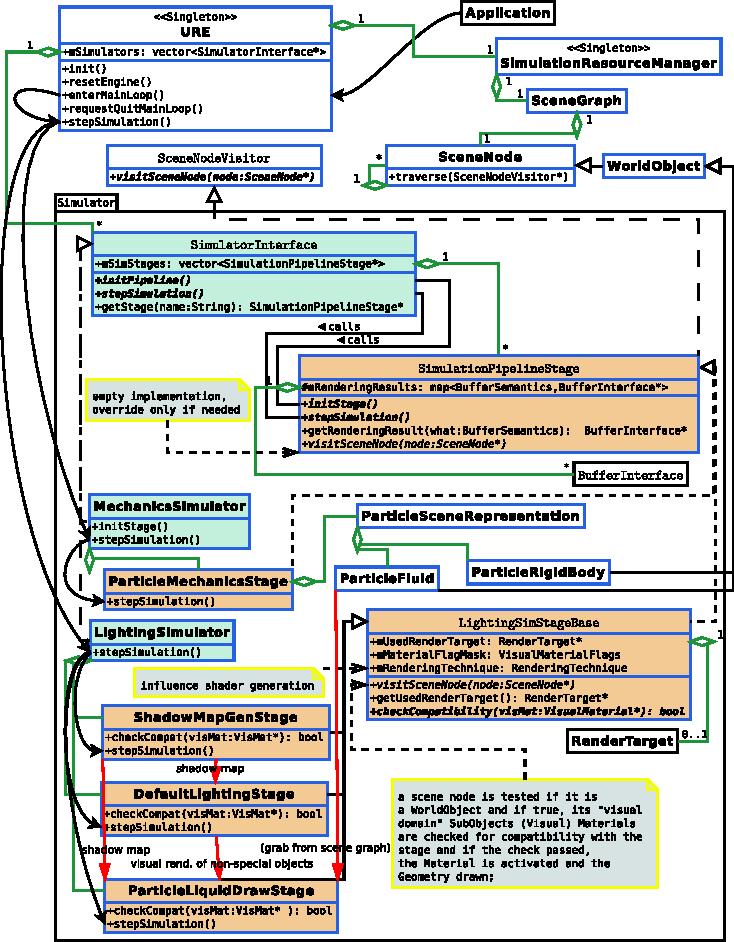
\includegraphics[width=1.15\textwidth]{Detail_Simulator.pdf}
	\caption{Grobes Beispiel von einer Simulation und den zugehörigen Daten-Abhängigkeiten}
	\label{fig:detailSimulator}
\end{figure}


Wie bereits erwähnt, soll jede Simulationsdömane einen eigenen Simulator haben, 
der eine eigene Pipeline an Simulations-Stages verwaltet.
Es kann theoretisch beliebig viele Simulationsdomänen geben. Momentan sind jedoch nur drei
über einen \lstinline|enum| definiert: Die visuelle, mechanische und akustische Domäne, wobei
die akustische Domäne noch nicht in der prototypischen Implementierung vorkommt.
Abb. \ref{fig:detailSimulator} zeigt grob beispielhaft den Ablauf einer Simulation und die verschiedenen
Varianten, wie man sich die "`Rendering Results"' anderer Stages beschaffen kann:\\
Entweder aus der Main Loop der Engine heraus oder von der benutzenden Applikation wird
\lstinline|URE::stepSimulation()| aufgerufen; Diese Funktion iteriert in fester Reihenfolge über die
vorhandenen Simulatoren und ruft deren \lstinline|stepSimulation()|-Routine auf; Hierin werden Simulator-
spezifische Operationen ausgeführt (Framebuffers des Fensters resetten und Haupt-Viewport setzen beim 
\lstinline|LightingSimulator|, CL/GL-shared Buffers für OpenCL akquirieren beim \lstinline|MechanicsSimulator|...),
dann über die einzelnen zugehörigen \linebreak
\lstinline|SimulationPipelineStage|'s iteriert, widerum deren 
\lstinline|stepSimulation()|-Methode aufgerufen.
Hier passiert dann das eigentlich \emph{generische Rendering}.
So verschieden die Algorithmen sind, die in den einzelnen Stages abgearbeitet werden, so verschieden sind auch
die Möglichkeiten, wie einzelne Stages miteinander Daten austauschen: Der generischste Ansatz ist, sich von einer
Stage einen Buffer mit einer bestimmten Semantik zu beschaffen, sofern die entsprechende Stage ein solchen
bereit stellt. Bei Lichtsimulation, die viel mit Texturen und OpenGL-Framebuffer-Objects (FBOs) umgeht,
bietet sich an, sich das \lstinline|RenderTarget| (die Abtraktion des FBO in \emph{Flewnit}) zu beschaffen,
um mit dem gesamten RenderTarget weiter zu arbeiten, oder sich einzelne Texturen zu beschaffen.
Es gibt aber auch die relativ indirekte Methode des Datenaustausches, wie es z.B. zwischen der 
\lstinline|ParticleMechanicsStage| und der \lstinline|ParticleLiquidDrawStage| der Fall ist: Die Buffer mit dem physikalischen Attributen sind in der SceneNode-abgeleiteten
Klasse \lstinline|ParticleFluid| enthalten, so dass die aktualisierten Daten über schlichtes Szenegraphen-Traversieren
beschafft werden können.\\
Details zum Ablauf der Simulation(en) werden in Kapitel \ref{sec:simulation} behandelt.




\subsection{Der SimulationResourceManger}
Diese Singleton-Klasse besitzt und verwaltet die Assets,\linebreak 
als \lstinline|std::map<String,X*>| für Referenzierung über einen Namen, 
wobei \lstinline|X| folgende Klassen betrifft: 
\begin{itemize}
	\item \lstinline|Material|
	\item \lstinline|Geometry|
	\item \lstinline|BufferInterface|
	\item \lstinline|Texture| \footnote{Da \lstinline|Texture| von \lstinline|BufferInterface| erbt, handelt es sich um 	
		eine Handle-Sammlung der Untermenge der Texturen aller \lstinline|BufferInterface|s, um einen bequemeren Zugriff zu 
		ermöglichen 
		}
	\item \lstinline|InstanceManager|
\end{itemize}
Außerdem bestitzt die Klasse den \lstinline|SceneGraph| und stellt einen Handle auf den aktuellen 
\lstinline|SkyDome| zur Verfügung, so dass alle Objekte ein konsistentes Environment Mapping 
betreiben können, sofern dies erwünscht ist.

		
\subsection{Das Scene-Paket}		
		

\subsection{Das WorldObject}
	Basis-Klasse fuer alles was unified simuliert wird: pure viuelle objekt, uniform grid, fluid, rigid body etc..
	
	\subsubsection{Das SubObject}
  
 
\subsection{Material}  
	was stellt welches material in welcher Domain dar?
	
\subsection{Geometry}
	Abtract, Buffer based, Vertex based etc.. ein paar konzepte (implementiert/genutzt nur VertexBased)  
	

    	
\subsection{Die Buffer-Abstraktion}  
	\label{sec:architecture:BufferAbstraction} 	
 	die bombe, die cpu, ogl und ocl vereint, inclusive ping ponging etc.. 
 	fundamentale Klassensammlung fuer den Unified-Aspekt
 	
 	\begin{figure}[!h]
  		\begin{tabular}
  		{
  		 l  l | c | c | c |
  		}
																	\cline{3-5}
  									&								&	\multicolumn{3}{ c | }{Context} \\ 
  																	\cline{3-5}
									&								& 	Host 	& 	OpenGL 	& 	OpenCL	\\
    	\noalign{\hrule}								
    	\multicolumn{1}{|c|}{
    		generic Buffer
    	}							& 								
    		&	{\color{green}\checkmark} 	&	{\color{red}x}		& 	{\color{green}\checkmark}	\\ 
    	
    	\noalign{\hrule}								
    	\multicolumn{1}{|c|}{
    		\multirow{4}{*}{OpenGL Buffers}
    	}							& Vertex Attribute Buffer		
    		&	{\color{orange}o} 	&	{\color{green}\checkmark}		& 	{\color{orange}o}	\\  
    								\cline{3-5}
    	\multicolumn{1}{|c|}{}		& Vertex Index Buffer			
    		&	{\color{orange}o} 	&	{\color{green}\checkmark}		& 	{\color{orange}o}	\\  
    								\cline{3-5}
    	\multicolumn{1}{|c|}{}		& Uniform Buffer
    		&	{\color{orange}o} 	&	{\color{green}\checkmark}		& 	{\color{orange}o}	\\ 
    								\cline{3-5} 
    	\multicolumn{1}{|c|}{}		& Render Buffer					
    		&	{\color{red}x} 	&	{\color{green}\checkmark}		& 	{\color{green}\checkmark}	\\ 
    
   		\noalign{\hrule}								
   		\multicolumn{1}{|c|}{
    		\multirow{4}{*}{Textures} 
   		}							& 1D Texture					
   			&	{\color{orange}o} 	&	{\color{green}\checkmark}		& 	{\color{red}x}	\\ 
    								\cline{3-5}
		\multicolumn{1}{|c|}{}		& 2D Texture				
			&	{\color{orange}o} 	&	{\color{green}\checkmark}		& 	{\color{green}\checkmark}	\\ 
									\cline{3-5}
		\multicolumn{1}{|c|}{}		& 3D Texture		
			&	{\color{orange}o} 	&	{\color{green}\checkmark}		& 	{\color{green}\checkmark}	\\ 
									\cline{3-5}
		\multicolumn{1}{|c|}{}		& Special Texture				
			&	{\color{orange}?} 	&	{\color{green}\checkmark}		& 	{\color{orange}?}	\\ 


    	\noalign{\hrule}
     
     	
  		\end{tabular}	
  	
  		\caption{		
  			Verschiedene Buffertypen und ihre Verfügbarkeit in verschiedenen Kontexten \\	
  			Legende: \\
			{\color{green}\checkmark}	$\rightarrow$ nativ unterstützt;
			{\color{orange}o}	$\rightarrow$ kompatibel;
			{\color{red}x}	$\rightarrow$ nicht unterstützt;	\\
			{\color{orange}?}	$\rightarrow$ Unterstützung abhängig von weiteren Parametern;	
		}
	
  	\end{figure}
 

\subsection{Das MPP-Paket}
Massively Parallel Program
	Basisklasse von Shader und OpenCL Program
	MPP und ParCompManager: hardware query, abstrakte methoden...
	\subsubsection{Shader}
		shader + manager+unterklassen
		
	\subsubsection{OpenCLProgram}
		shader + manager+unterklassen + arguments etc.. event waiting, synch, acquire...

weitere klassen/konzepte to go...	?


\subsection{Status der Implementierung am Ende der BA}
	
	Features auflisten;
	\todo[color=green]{screenshots? oder lieber erst später,zusammen mit detaillierter erläuterung?}

	großteils programmierte, aber ungenutzte/ungetestete features erwähnen (Deferred Rendering, Layered Rendering, 	
	RenderTarget-Klasse, Partikel-Rigid bodies, verschiedene Fluid-Typen); 


	überlegte aber nciht programmierte Konzepte/Algorithmen erwähnen (Triangle-Index-Voxelisierung)
	
	schlimmste schnitzer nennen, wie
		- miese fluid-visualisierung, 
		- unübersichtliche shadertemplates, besser gemacht bei CL-
			Kernel-Templates, 1. weil struktur hier besser "vererbbar", 2. weil mehr erfahrung mit  Template-Engine
	
	  	
  	

\clearpage
